\section{Generative Adversarial Networks}

Until now the models we explored failed to capture complex, high-dimensional data types (e.g. images and audio). The key idea is to use a neural network to learn a function that takes a "simple" distribution (e.g. Gaussian) and returns a non linear distribution. This leads us to the problem that it becomes to compute the likelihood of the data needed for the loss. Therefore we need an alternative objective for training.

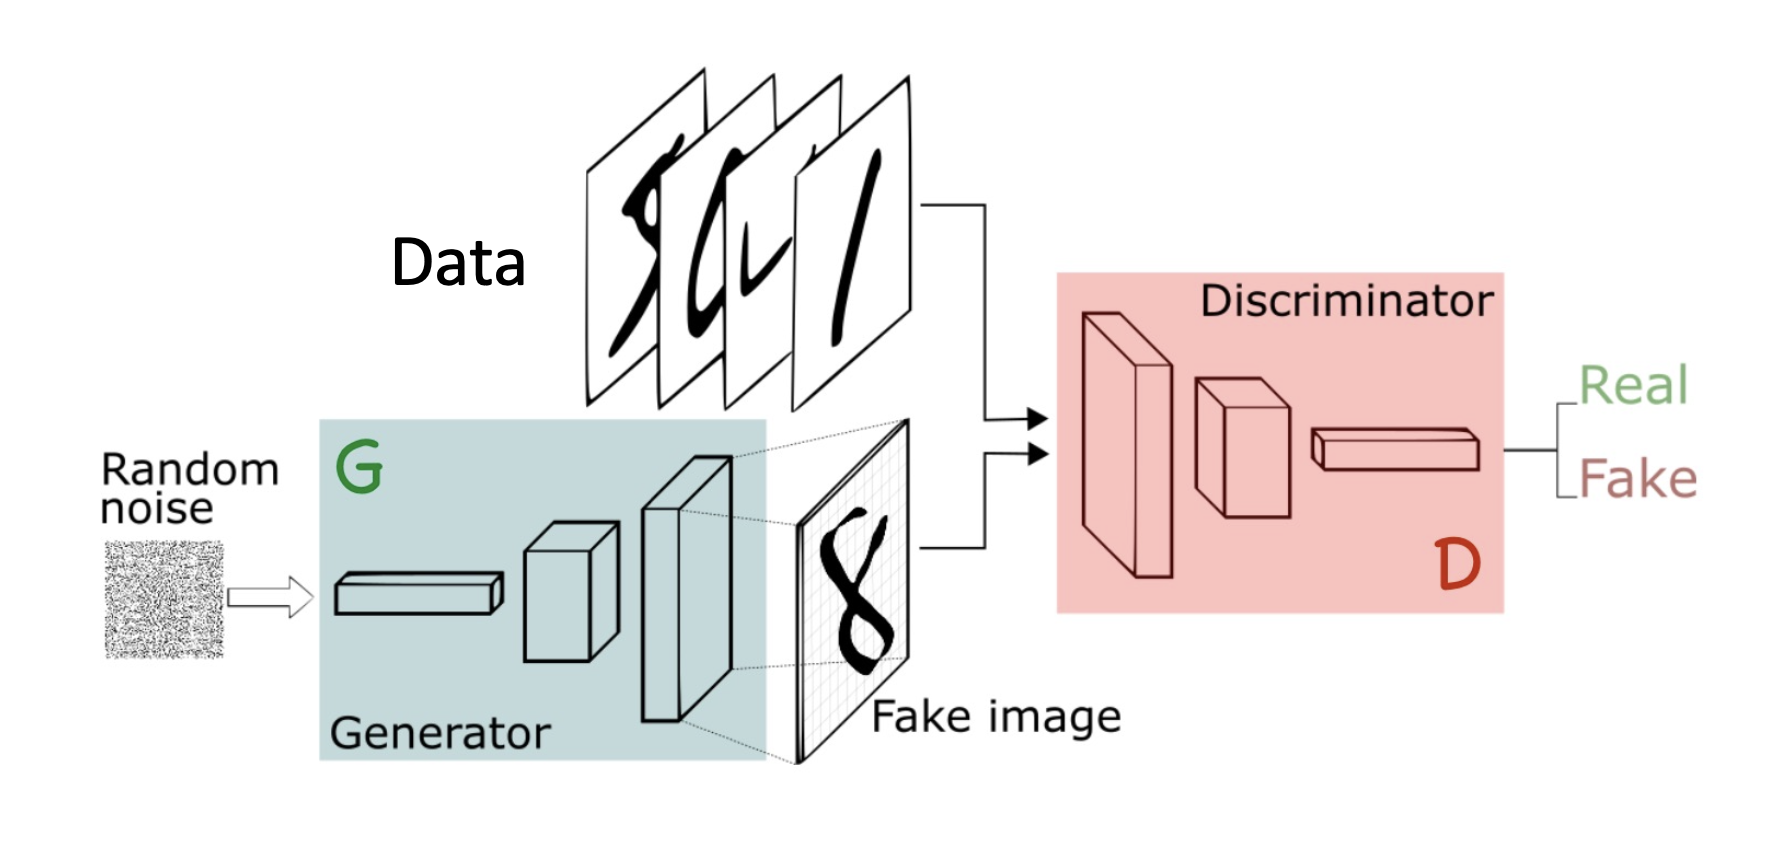
\includegraphics[width=\columnwidth]{gan.png}

We simultaneously train two neural networks, a generator $G$ trying to produce realistic examples and a discriminator $D$ trying to detect "fake" examples. This whole process can be viewed as a game, where the generator and discriminator try to compete against each other. This leads to the following objective:

\begin{align*}
	\min_{w_G} \max_{w_D} \; & \E_{x \sim p_{\text{data}}} [\log D(x, w_D)] \\
 	+ &\E_{z \sim p_z} [\log (1 - D(G(z, w_G), w_D))]
 \end{align*}
 
 Training a GAN requires to find the saddle point rather than a (local) minima. For a fixed generator $G$, the optimal discriminator is such that:
 $$D_G(x) = \frac{p_{\text{data}}(x)}{p_{\text{data}}(x) + p_G(x)}$$
 
 In general it is important that the discriminator is not too powerful, as this could lead to memorization on finite data. Other issues that can occur are oscillations/divergence or mode collapse. \medskip
 
 Evaluation GANs is still an open research question. One possible performance metric is the so called duality gap:
 $$DG(w_G, w_D) = \max_{w_D'} M(w_G, w_D') - \min_{w_G'} M(w_G', w_D)$$
 
 Where $M(w_G, w_D)$ is the objective used in training.